\documentclass[12pt]{article}

\usepackage[english]{babel}
\usepackage[utf8]{inputenc}
\usepackage{amsmath}
\usepackage{commath}
\usepackage{booktabs}
\usepackage[alf]{abntex2cite}
\usepackage{indentfirst}
\usepackage{graphicx}
\usepackage{multicol,lipsum}
\usepackage{geometry}
\usepackage[alf]{abntex2cite}
\usepackage{siunitx}
%\usepackage[scriptsize]{subfigure}
%\usepackage{caption}
\usepackage{subcaption}
\graphicspath{{../../Figures/Report_20_01/}{../../Images/Report_20_01/}}

\geometry{
  paper = a4paper,
  inner = 3cm,
  outer = 3cm,
  top = 2cm,
  bottom = 2cm
}

\usepackage{tabularx}

\renewcommand{\baselinestretch}{1.5} 

\begin{document}
%\maketitle

\begin{titlepage}
\begin{center}

\Huge{Universidade Federal de Alagoas}\\
\large{Instituto de Computação}\\ 
\large{Laboratório de Computação Científica e Análise Numérica}\\ 
\vspace{220pt}
\textbf{\LARGE{Research report}}\\
%\title{{\large{Título}}}
\vspace{3,5cm}
\end{center}

\begin{flushleft}
\begin{tabbing}
Student: Danilo Fernandes Costa\\
Professor: Alejandro Frery\\
\end{tabbing}
\end{flushleft}
\vspace{1cm}

\begin{center}
\vspace{\fill}
January\\
2020
\end{center}
\end{titlepage}

\section{Introduction}
%Descrever Roteiro da análise: Descrever os dados selecionados (com imagens na decomposição de Pauli), Análise descritiva (histogramas e boxplots), Ajuste, Teste de separabilidade (Anova) 

In this report, we analyse five PolSAR images of the same region -- a soilbeans crop -- obtained over time, which were disponibilized by Avik Bhattacharya and his research group. The first image was made on 16 May 2016, which was followed by four others at time intervals of 24 days. These images, through Pauli Decomposition, are shown in the figure \ref{fig:sample_images}. 

\begin{figure}[hbt]
  \centering
  \subcaptionbox{16 May 2016\label{fig:day_0}}{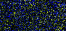
\includegraphics[width = .19\linewidth]{sb231_day_0}}
  \subcaptionbox{09 June 2016\label{fig:day_24}}{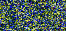
\includegraphics[width = .19\linewidth]{sb231_day_24}}
  \subcaptionbox{03 July 2016\label{fig:day_48}}{
\includegraphics[width = .19\linewidth]{sb231_day_48}}
  \subcaptionbox{27 July 2016\label{fig:day_72}}{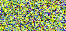
\includegraphics[width = .19\linewidth]{sb231_day_72}}
  \subcaptionbox{20 Aug. 2016\label{fig:day_96}}{
\includegraphics[width = .19\linewidth]{sb231_day_96}}
  \caption{Sample analyzed over time}
  \label{fig:sample_images}
\end{figure}

The roadmap for the data analysis of these images followed as follows:
\begin{itemize}
  \item Obtaining the geodesic purity index of the data;
  \item Descriptive analysis of the data by image through histograms and boxplots;
  \item Fitting of histograms to known probability distributions;
  \item Separability test through Analysis of Variance.
\end{itemize}

The geodesic purity index measures the distance between a target and the ideal depolarizer. This is, as a Kennaugh matrix, given by:

{\setstretch{1.0}
\[ \mathbf{K}_{dep} =
\begin{bmatrix}
1 & 0 & 0 & 0\\
0 & 0 & 0 & 0\\
0 & 0 & 0 & 0\\
0 & 0 & 0 & 0
\end{bmatrix}.
\]
}
The geodesic purity index is calculated as follows:
\begin{equation}
  P_{GD} = \left(\frac{3}{2}GD(\mathbf{K}, \mathbf{K}_{dep})\right)^2
\end{equation}

\section{Data analysis}

After calculating the purity for the analyzed dataset, histograms and boxplots were obtained from the logarithm of the calculated indices for each image, which are shown in the figure \ref{fig:histograms}. Through this graph, one can suppose that these data obey a Normal distribution. To graphically analyze this, the respective qqplots were produced, which are shown in the figure \ref{fig:qqplots}. It can be seen that these graphs are compliant with the supposition.

\begin{figure}[hbt]
  \centering
  \subcaptionbox{Histograms\label{fig:histograms}}{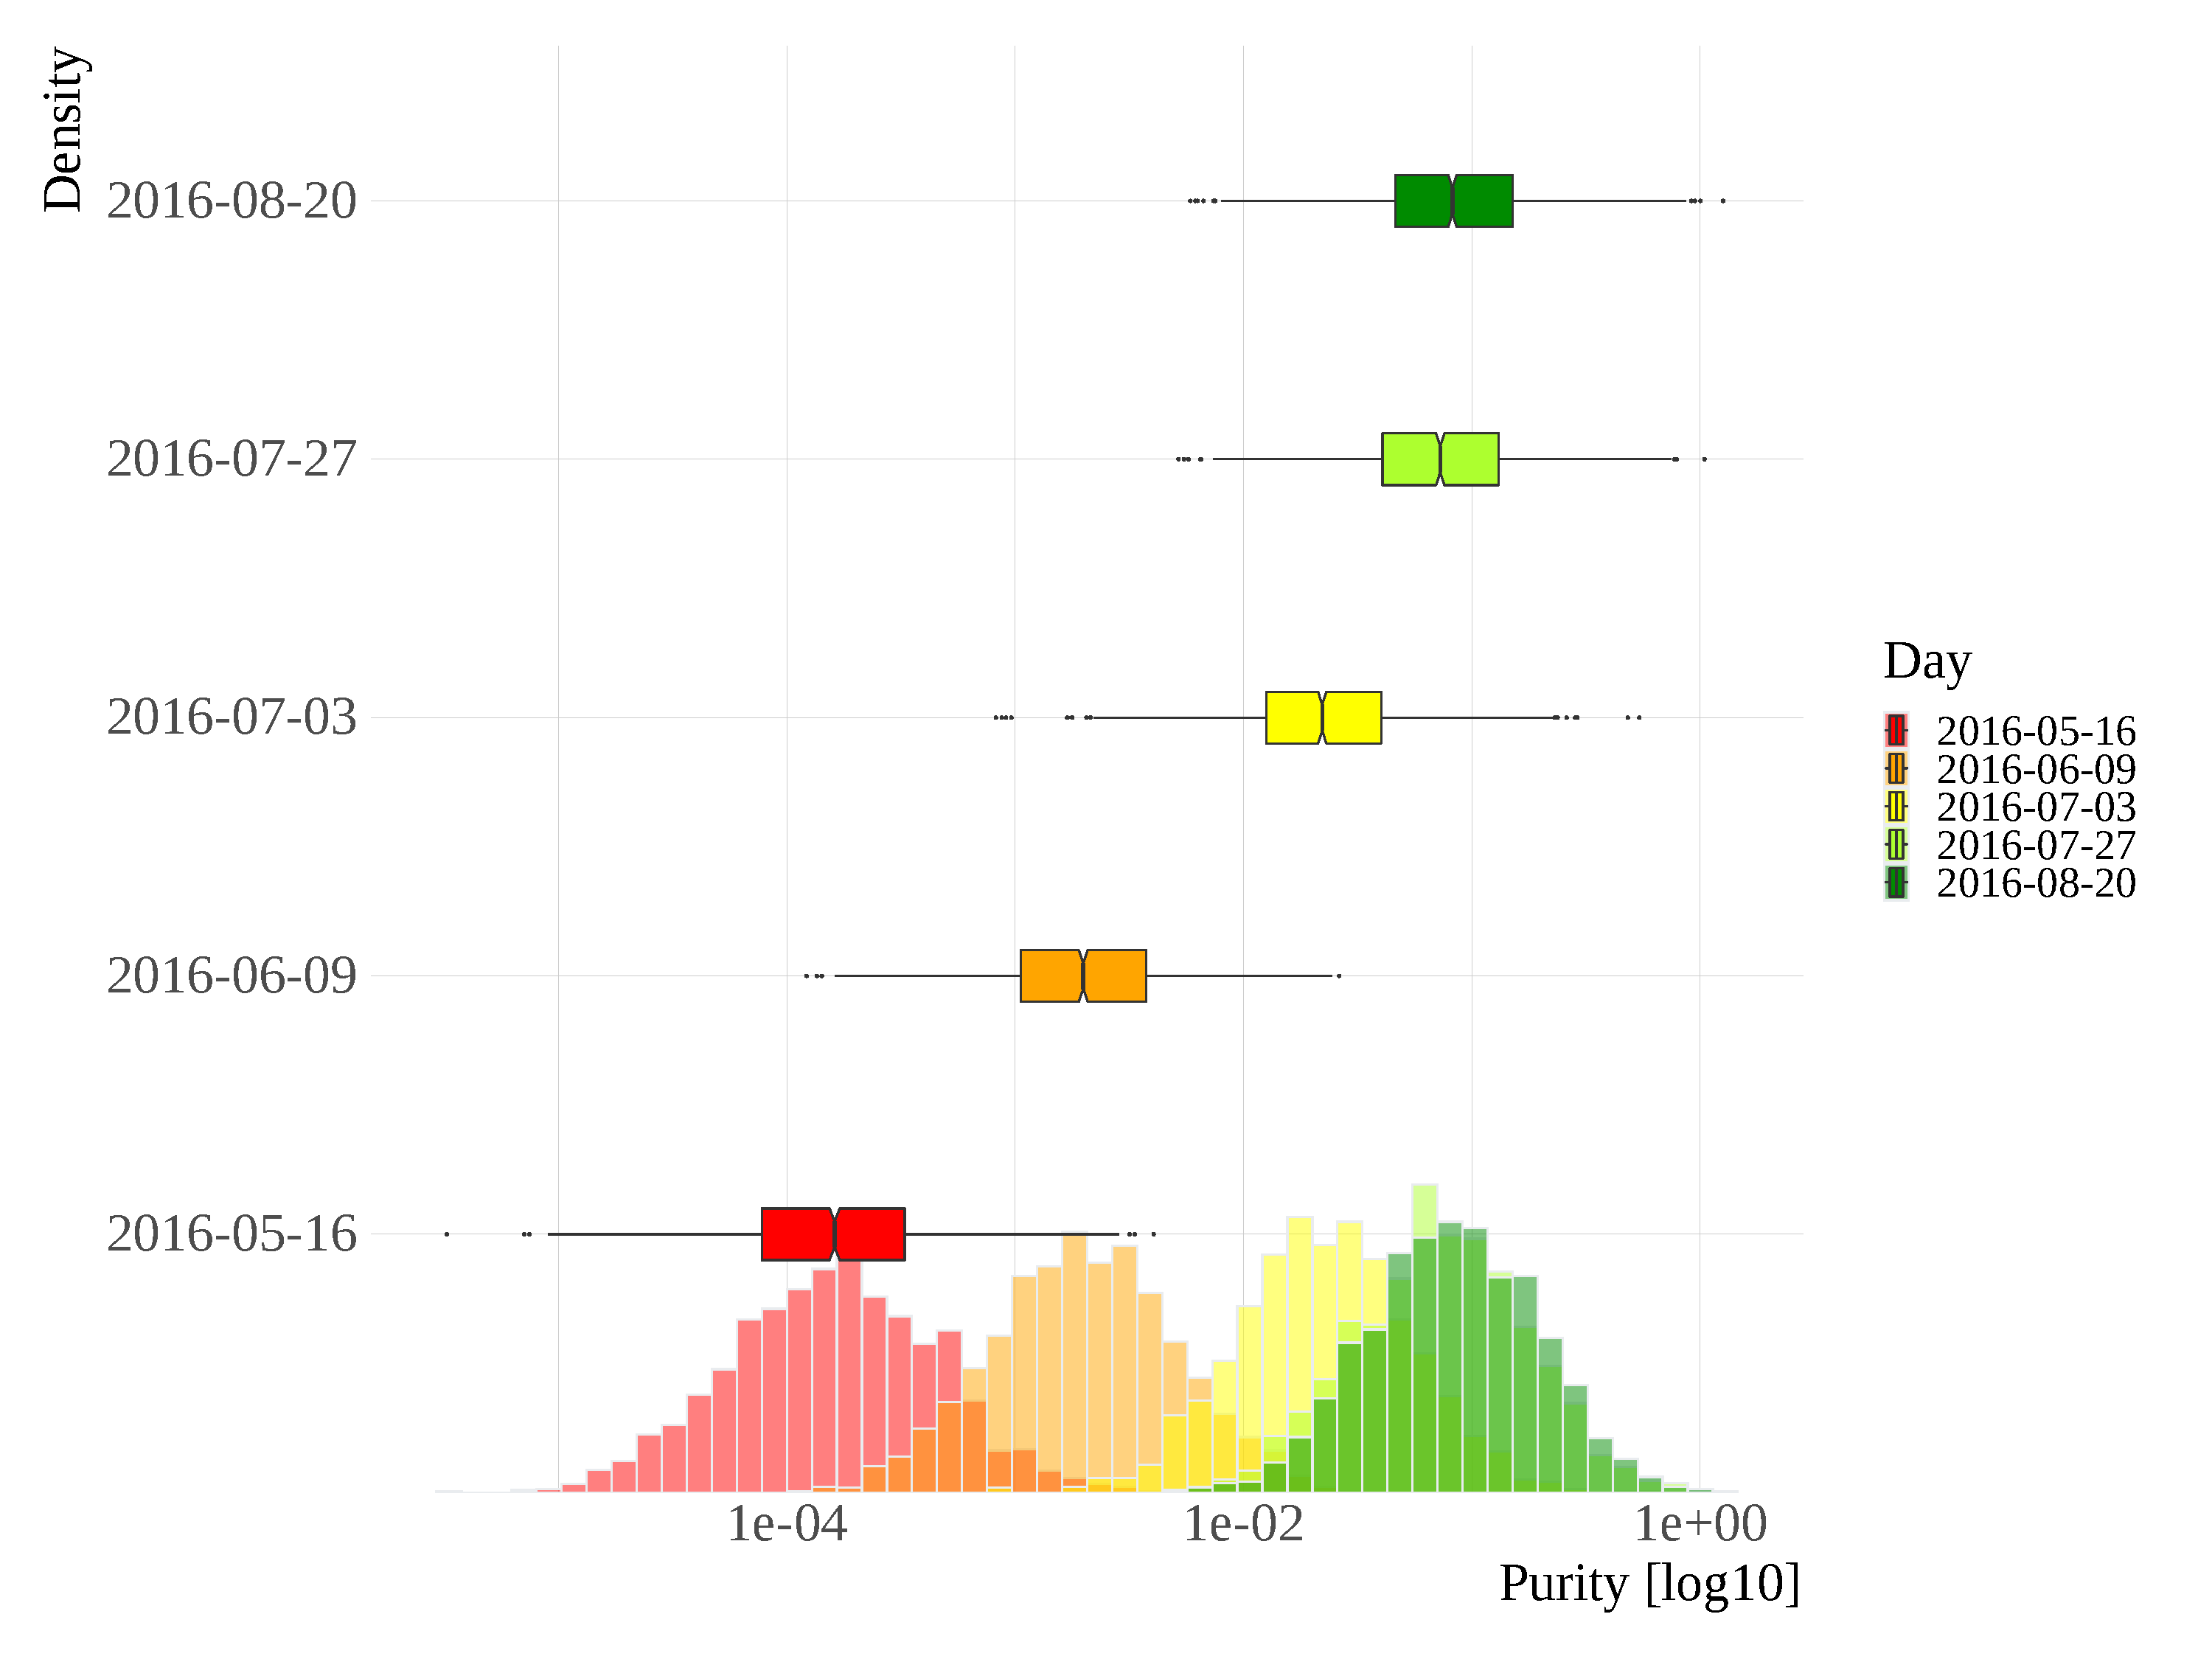
\includegraphics[width = .49\linewidth]{histograms}}
  \subcaptionbox{QQPlots\label{fig:qqplots}}{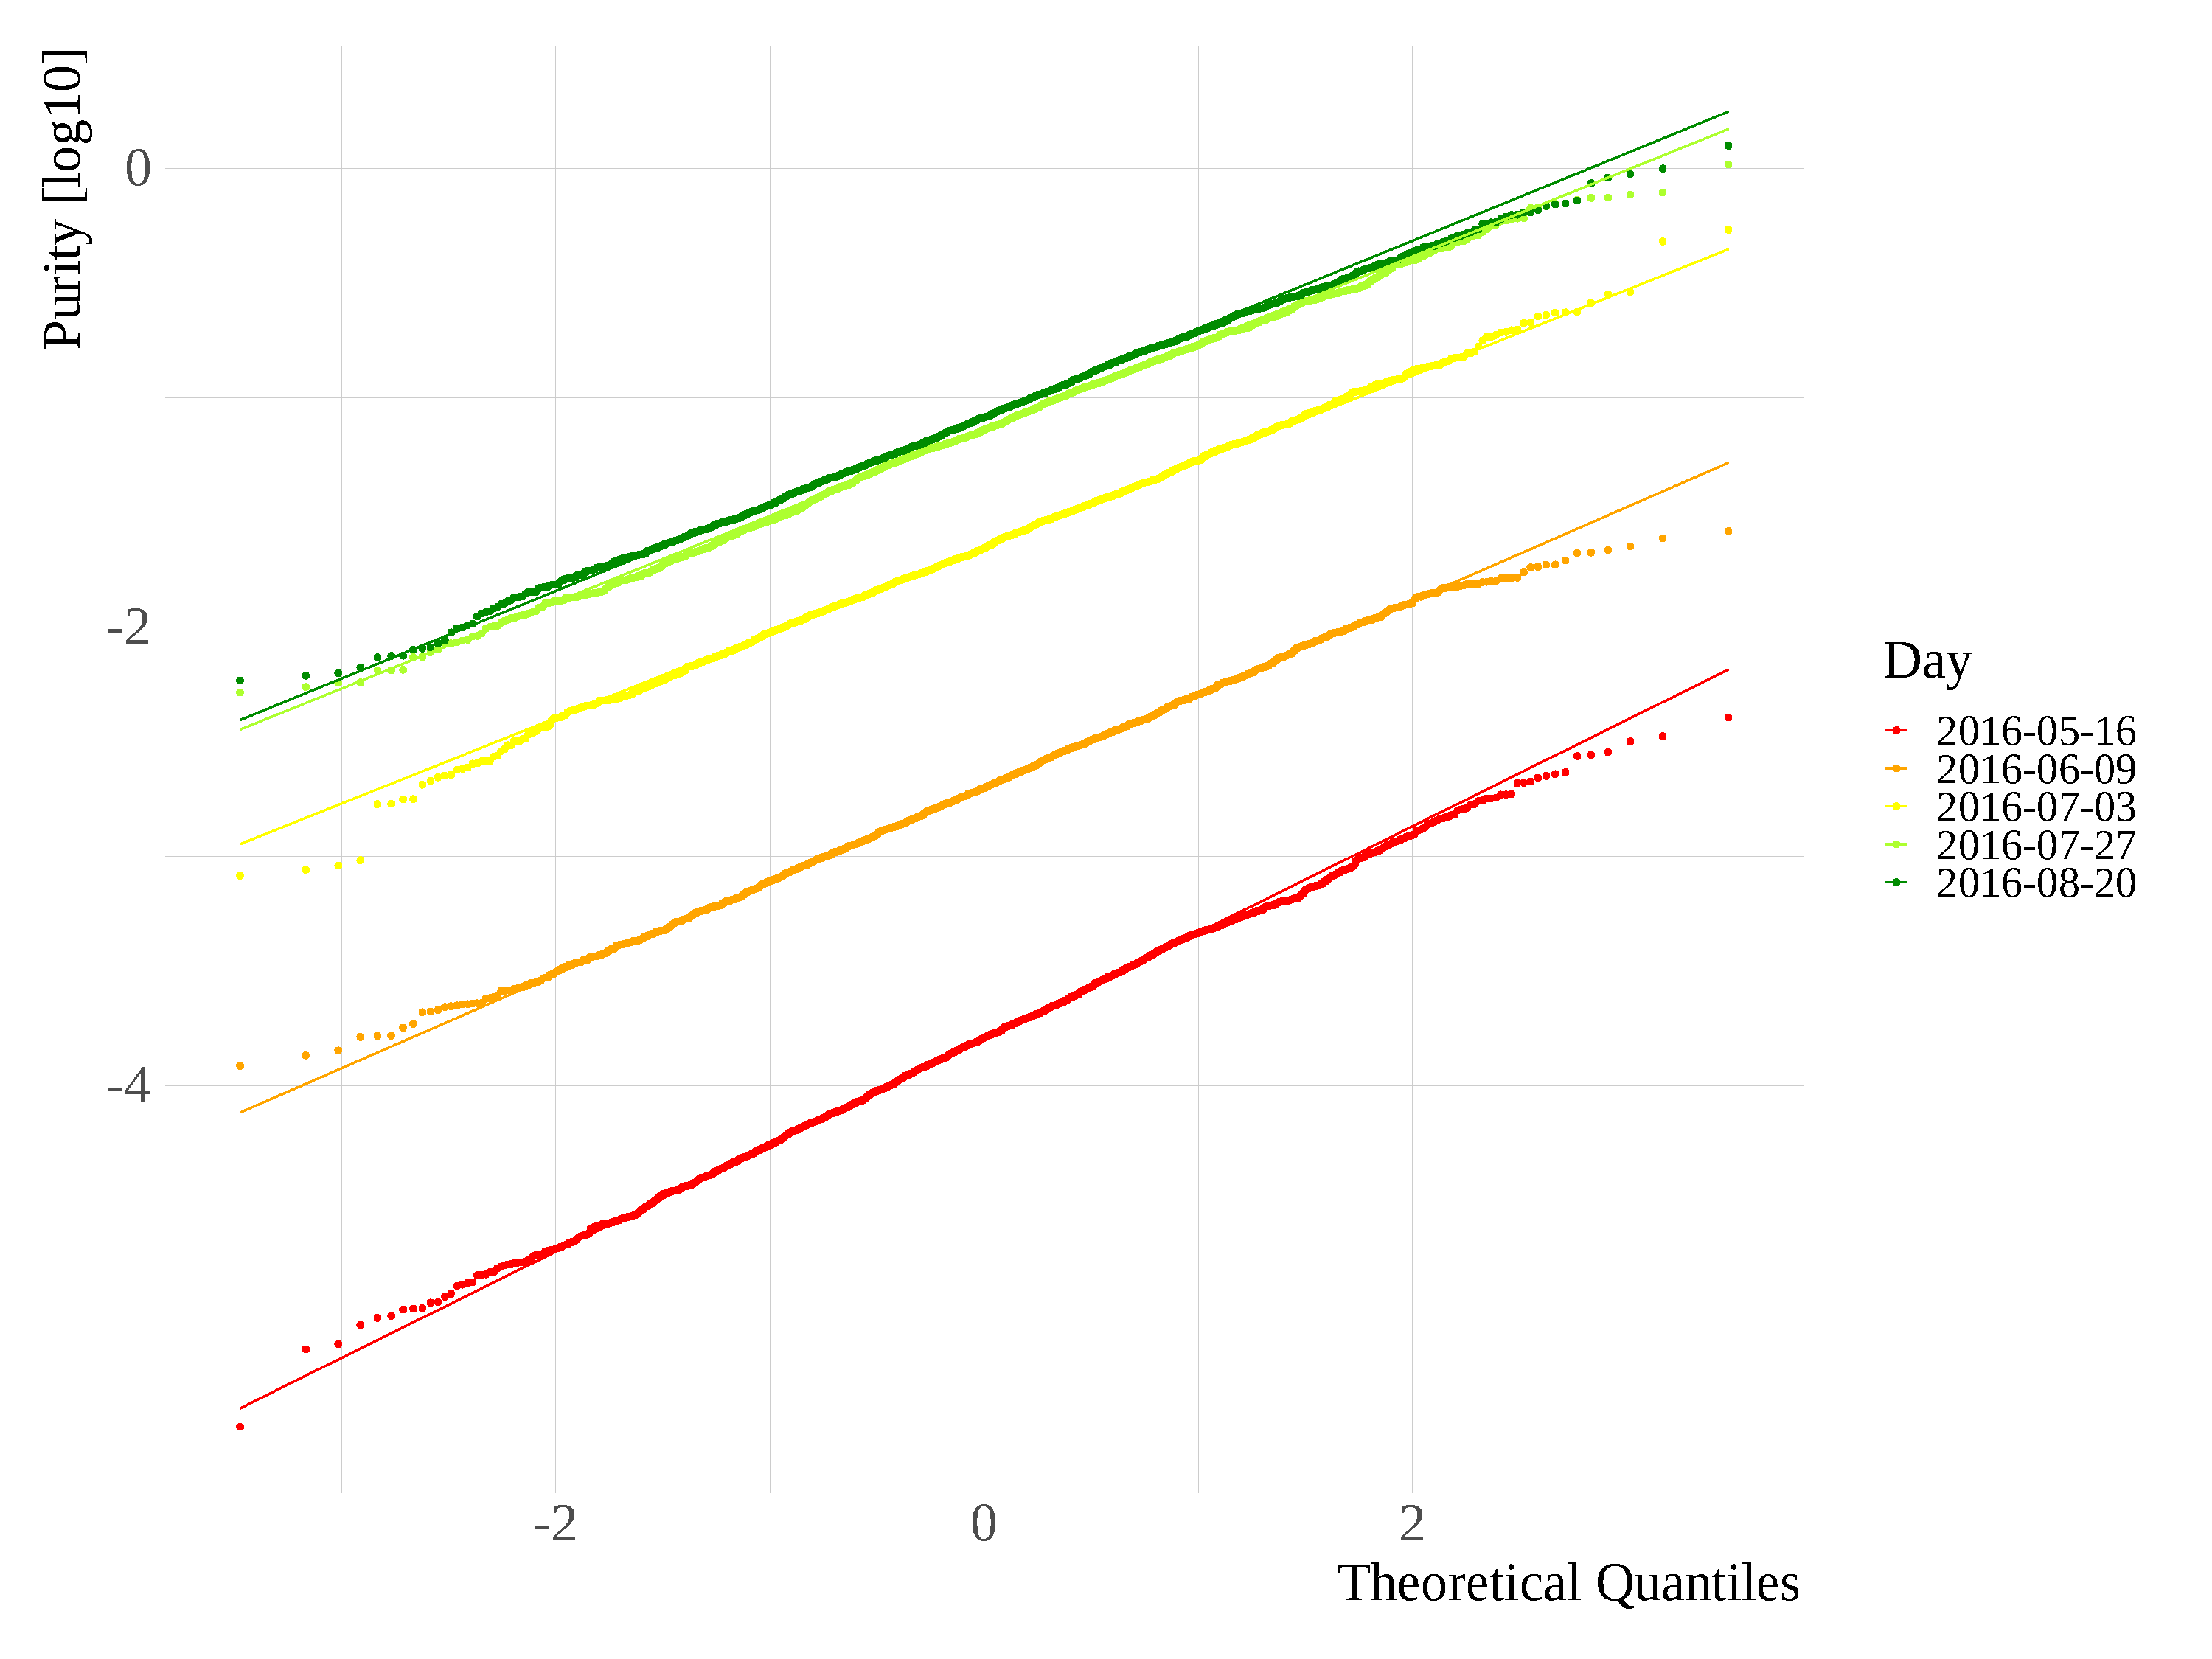
\includegraphics[width = .49\linewidth]{qqplots}}
  \caption{Descriptive analysis of the logarithm of the calculated purity values for each image}
  \label{fig:desc_analysis}
\end{figure}

Based on this assumption, normality tests (Shapiro-Wilk test) were performed from which the $p$-values are in the table \ref{tab:pvalues}. From these, it is possible to conclude that, at the level of $0.05$, it is not possible to reject the null hypothesis that these data obey the normal distribution. 

\begin{table}[hbt]
  \centering
  \caption{$p$-values from Shapiro-Wilk Test}
  \label{tab:pvalues}
  \begin{tabular}{rrrrr}
    \toprule
    \textbf{Day 0} & \textbf{Day 24} & \textbf{Day 48} & \textbf{Day 72} & \textbf{Day 96}\\
    0.4963 & 0.0650 & 0.3494 & 0.0585 & 0.3919\\
    \bottomrule
  \end{tabular}
\end{table}

\end{document}